\chapter{Tecnologias disponíveis} \label{Tecnologias disponíveis}

\section{Linguagens de Programação}

Uma linguagem de programação é a forma que os programadores utilizam como meio de comunicação com os computadores. A lógica necessária para o funcionamento de um programa é convertida em um conjunto de caracteres seguindo um conjunto de regras sintáticas e semânticas que formará um código ou \textit{script}.

\subsection{As linguagens disponíveis}

Assim como os idiomas falados são muitos, o número de linguagens de programação disponíveis também é alto, com isso, um desenvolvedor deverá saber escolher qual linguagem utilizar dependendo do tipo do projeto que será desenvolvido. Um critério que poderá ser utilizado para essa escolha é o grau de popularidade que uma linguagem de programação possui entre a comunidade de programadores.

A contabilização da popularidade dessas linguagens é feita por algumas instituições no qual um programador poderá se basear para efetuar sua escolha. Caso o mesmo não possua domínio daquelas mais populares poderá utilizar como critério para aprendizado e se reciclar perante ao mercado assim como um médico deve sempre se atualizar a cura de novas doenças antes não disponíveis durante o seu período de estudos acadêmicos.

Através do índice TIOBE é possível obter o grau de popularidade das linguagens de programação. O índice é elaborado através dos resultados dos sites de buscas por essas mesmas linguagens seguindo alguns critérios adotados pela empresa TIOBE Software BV a qual mantém elabora o mesmo. Vale ressaltar que esse índice é divulgado mensalmente, sendo possível obter informações históricas da popularidade das linguagens através de soluções pagas oferecidas por essa mesma empresa.

A \autoref{tab-tiobe} ilustra as 20 linguagens mais populares de acordo com esse índice. Esses dados foram gerados a partir de um levantamento realizado no início dos anos de 2020 e 2019 e tendo sido divulgados nos meses de fevereiro dos respectivos anos.

% FIXME: Verificar ABNT se pode centralizar
\begin{table}[htb]
\ABNTEXfontereduzida
\caption[Índice TIOBE]{Índice TIOBE.}
\label{tab-tiobe}
\begin{tabular}{p{2.6cm}|p{2.6cm}|p{4cm}}
  %\hline
   \textbf{Fevereiro/2020} & \textbf{Fevereiro/2019}  & \textbf{Linguagem}  \\
    \hline
    1 & 1 & Java \\
    \hline
    2 & 2 & C \\
    \hline
    3 & 3 & Python \\
    \hline
    4 & 4 & C++ \\
    \hline
    5 & 7 & C\# \\
    \hline
    6 & 5 & Visual Basic .NET \\
    \hline
    7 & 6 & JavaScript \\
    \hline
    8 & 8 & PHP \\
    \hline
    9 & 9 & SQL \\
    \hline
    10 & 20 & Swift \\
    \hline
    11 & 18 & Go \\
    \hline
    12 & 11 & Assembly Language \\
    \hline
    13 & 15 & R \\
    \hline
    14 & 23 & D \\
    \hline
    15 & 16 & Ruby \\
    \hline
    16 & 12 & MATLAB \\
    \hline
    17 & 21 & PL/SQL \\
    \hline
    18 & 14 & Delphi/Object Pascal \\
    \hline
    19 & 13 & Perl \\
    \hline
    20 & 10 & Objective-C \\
\end{tabular}
\legend{Fonte: \citeonline{tiobeDefinition}}
\end{table}

\newpage
Uma outra instituição que efetua ranking semelhante é o Stack Overflow, uma empresa fundada em 2008 na qual possui maior comunidade de desenvolvedores para compartilhamento do conhecimento relacionado com programação. Essa comunidade dar-se em torno de um site utilizado para troca de conhecimento de forma colaborativa através da ajuda na resolução de problemas e desmistificação de dúvidas.

% FIXME: Melhorar esse trecho. Generalizar pesquisa. Esmiuçar ranking depois.
O ranking elaborado por essa empresa é divulgado de forma anual através de uma pesquisa, no próprio site, com programadores de todo mundo. Para versão referente ao ano de 2019, foram entrevistados aproximadamente 90.000 desenvolvedores. Esse mesmo ranking pode ser observado na \autoref{tab-stack-overflow-linguagens}.

% FIXME: Acrescentar mais detalhes do ranking.

% FIXME: Verificar ABNT se pode centralizar
\begin{table}[htb]
\ABNTEXfontereduzida
\caption[Ranking das Linguagens Mais Populares]{Ranking das Linguagens Mais Populares.}
\label{tab-stack-overflow-linguagens}
\begin{tabular}{p{5cm}|p{4cm}}
  %\hline
   \textbf{Linguagem} & \textbf{Porcentagem de uso}  \\
    \hline
    JavaScript & 69,7\%  \\
    \hline
    HTML/CSS & 63,1\%  \\
    \hline
    SQL & 56,5\%  \\
    \hline
    Python & 39,4\%  \\
    \hline
    Java & 39,2\%  \\
    \hline
    Bash/Shell/PowerShell & 37,9\%  \\
    \hline
    C\# & 31,9\%  \\
    \hline
    PHP & 25,8\%  \\
    \hline
    TypeScript & 23,5\%  \\
    \hline
    C++ & 20,4\%  \\
    \hline
    C & 17,3\%  \\
    \hline
    Ruby & 8,9\%  \\
    \hline
    Go & 8,8\%  \\
    \hline
    Swift & 6,8\%  \\
    \hline
    Kotlin & 6,6\%  \\
    \hline
    R & 5,6\%  \\
    \hline
    VBA & 5,5\%  \\
    \hline
    Objective-C & 5,2\%  \\
    \hline
    Assembly & 5,0\%  \\
    \hline
    Scala & 4,2\%  \\
    \hline
    Rust & 3,0\%  \\
    \hline
    Dart & 1,8\%  \\
    \hline
    Elixir & 1,6\%  \\
    \hline
    Clojure & 1,5\%  \\
    \hline
    WebAssembly & 1,1\%  \\
\end{tabular}
\legend{Fonte: \citeonline{stackOverflowRanking}}
\end{table}

\newpage
Conforme pode ser observado na \autoref{tab-stack-overflow-linguagens}, existe uma intersecção de linguagens populares entre os dois rankings.

A linguagem de programação JavaScript aparece bem colocada em ambos os rankings, no índice TIOBE na sexta posição e na liderança do Ranking do StackOverflow. Conforme será destacado na seção \ref{JavaScript}, essa linguagem pode ser utilizada para diversos tipos de aplicação, como por exemplo o seu uso mais comum, isto é, em navegadores, assim como para o uso em servidores e até mesmo para desenvolvimento de aplicativos para dispositivos móveis.

\section{Desenvolvimento para dispositivos móveis}
\label{sec-desenvolvimento-apps}

O uso de \textit{smartphones} tornou-se popular com a criação do \textit{iPhone}, desenvolvido pela \textit{Apple}, em 2008. Mais de 10 anos após o lançamento da primeira versão, os ditos celulares inteligentes estão cada vez mais modernos e mais populares.

%% Acrescentar tabela evolução celulares e consumo, vendas

Os sistemas operacionais para dispositivos móveis mais populares são o IOS e o Android, sendo o primeiro exclusivo de aparelhos fabricados pela Apple, já o segundo é um sistema composto por código aberto sendo que um do seus principais mantedores é o Google e é utilizado por diversas empresas como Samsung, Motorola, LG, Xiaomi, Huawei e outras.

O desenvolvimento para esses sistemas possui certas particularidades, sendo que para o sistema da empresa fundada por Steve Jobs utiliza como linguagens de programação para desenvolvimento nativo o Swift e o Objective-C, já o sistema mantido pela empresa de Mountain View utiliza a linguagens Java e Kotlin.

De forma a aumentar o alcance de um aplicativo, o programador deve disponibilizar o mesmo nessas duas plataformas. Como é possível observar, não existe uma intersecção de linguagens disponíveis para o desenvolvimento nativo para essas plataformas, logo, o mesmo aplicativo deveria ser programado de duas formas diferentes, isto é, utilizando no mínimo duas linguagens de programação, fazendo com que mais tempo fosse necessário durante o desenvolvimento, pois seria necessário construir a mesma coisa duas vezes. Para contornar esse problema, alternativas foram desenvolvidas para otimizar o tempo de desenvolvimento, ou seja, o programador desenvolveria um código e esse mesmo poderia ser utilizado para os dois sistemas. Essa técnica é denominada de Desenvolvimento Multiplataforma (\textit{Cross-Platform}).

O Desenvolvimento Multiplataforma pode ser efetuado de duas formas, "Hybrid" e "Native". O primeiro utiliza recursos de desenvolvimento Web, como HTML, JS e CSS para a construção da aplicação pois a mesma será executada a partir de um navegador, já o segundo faz o usufruto de Frameworks que iram gerar arquivo compilado como se fosse nativo para cada plataforma, sendo que a linguagem utilizada varia com o Framework escolhido. Além disso, para essa última solução é possível mesclar código nativo com o desenvolvido pelo Framework.

Alguns exemplos de Frameworks utilizados em soluções de desenvolvimento "Hybrid" são o Cordova, Ionic e PhoneGap, já para as soluções do tipo "Native" podem serem citados como exemplo o Flutter, React Native e o Xamarim.

As aplicações quando desenvolvidas utilizando esses três últimos Frameworks descritos anteriormente fornecem uma performance melhor quando comparadas àquelas aplicações desenvolvidas com os três primeiros.

Vale ressaltar que há uma preferência no mercado para o uso dos Frameworks dessa última solução apresentada. Essa afirmação pode ser observada após uma breve análise da \autoref{tab-stack-overflow-framework-tools}, pois o React Native possui uma parcela maior do mercado quando comparado ao Cordova também presente na mesma tabela. Além desses, também está presente o Framework Flutter, tendo sido lançado a menos tempo quando comparado a esses outros dois.

Portanto, deve ser observado que as linguagens utilizadas por esses Frameworks de Desenvolvimento Multiplataforma "Native" são Dart, JavaScript e C\#, respectivamente para, Flutter, React Native e Xamarim.

\section{JavaScript}\label{JavaScript}

Antes as páginas eram construídas de modo estático, isto é, caso o usuário inserisse um conjunto de informações em um formulário, e caso, dentre esse conjunto, contivesse um dado inválido, a validação era feita do lado do servidor (Server Side) e dependendo da forma em que o site foi construído, toda informação inserida pelo usuário poderia ser perdida, necessitando que o mesmo as inserissem novamente.

De forma a corrigir esse problema e melhorar a navegação das páginas para tornar a experiência do usuário mais agradável, eis que surge a linguagem de programação JavaScript por volta do fim do ano de 1995, algo que revolucionou as páginas dessa mesma época.

Com o JavaScript, uma linguagem interpretada, é possível tornar as páginas da Web dinâmicas, além de que o problema da perda de informação de formulários poderia ser facilmente corrigido com o uso dessa linguagem.

A validação que antes necessitava de uma nova requisição com o servidor, agora poderia ser feito no próprio lado do cliente (Client Side), ou seja, a partir de um script que poderia ser executado no próprio navegador do usuário, o que poderia efetuar a mesma verificação de dados com a mesma precisão de antes.

Além disso, por estar executando na própria máquina do cliente, o processo torna-se muito mais rápido, pois pode ser feito instantaneamente após o usuário terminar de inserir uma determinada informação, não sendo necessário inserir todas as informações necessárias ao formulário para então efetuar a verificação.

Outra vantagem, é que esse procedimento é muito mais rápido em decorrência do tempo de processamento ser diminuído uma vez que não é mais necessário efetuar novas requisições de validações ao servidor, logo, não ocorrerá mais atraso no tempo de execução tendo a latência da comunicação entre a máquina do cliente com o servidor como causa.

Vale destacar a latência desse período era muito maior quando comparada aos dias atuais, pois a conexão com a internet ainda era feita de modo discado, isto é, conectando-se a rede mundial de computadores por meio do telefone.

\subsection{A Popularidade do JavaScript}
\label{secao-javascript-popularidade}

Como é possível observar no ranking das linguagens, elaborado pelo StackOverflow, no qual é representado pela \autoref{tab-stack-overflow-linguagens}, a linguagem JavaScript foi a mais popular nessa pesquisa. Isso pode ser justificado pois além do uso em seu propósito inicial, isto é, para uso em navegadores, essa linguagem também está sendo utilizado para programação de servidores web, criação de programas para computadores e até mesmo para construção de aplicativos móveis. Essa flexibilidade no uso da linguagem é possível com a utilização de Frameworks.

Esse comportamento fica evidente após uma análise da \autoref{tab-stack-overflow-framework-tools} que representa o ranking a respeito dos "Frameworks, Bibliotecas e Ferramentas Mais Populares". Esse ranking foi elaborado através das respostas de 49.861 desenvolvedores que fazem usufruto desses recursos para o meio profissional. Na liderança, sendo utilizado em 50,4\% dos casos, consta o Framework "Node.js" que é utilizado na criação de servidores com o JavaScript. Outro framework utilizado com essa mesma linguagem também presente no Top 5, é o "React Native" que é utilizado para o desenvolvimento de aplicações móveis.

Os outros três frameworks mais populares, isto é, ".Net", ".Net Core" e "Pandas" são utilizados com outras linguagens também populares sendo os dois primeiros utilizados com o "C\#" e o último com o "Python".

% FIXME: Verificar ABNT se pode centralizar
\begin{table}[htb]
\ABNTEXfontereduzida
\caption[Ranking dos Frameworks, Bibliotecas e Ferramentas Mais Populares]{Ranking dos Frameworks, Bibliotecas e Ferramentas Mais Populares.}
\label{tab-stack-overflow-framework-tools}
\begin{tabular}{p{5cm}|p{4cm}}
  %\hline
   \textbf{Frameworks, Bibliotecas e Ferramentas} & \textbf{Porcentagem de uso}  \\
    \hline
    Node.js & 50,4\%  \\
    \hline
    .NET & 38,1\%  \\
    \hline
    .NET Core & 24,5\%  \\
    \hline
    Pandas & 12,3\%  \\
    \hline
    React Native & 10,8\%  \\
    \hline
    Ansible & 10,4\%  \\
    \hline
    TensorFlow & 9,4\%  \\
    \hline
    Unity 3D & 9,1\%  \\
    \hline
    Cordova & 7,4\%  \\
    \hline
    Xamarin & 6,5\%  \\
    \hline
    Apache Spark & 5,9\%  \\
    \hline
    Hadoop & 5,0\%  \\
    \hline
    Flutter & 3,2\%  \\
    \hline
    Torch/PyTorch & 2,9\%  \\
    \hline
    Puppet & 2,9\%  \\
    \hline
    Chef & 2,7\%  \\
    \hline
    Unreal Engine & 2,6\%  \\
    \hline
    CryEngine & 0,4\%  \\
    
\end{tabular}
\legend{Fonte: }
\end{table}

% FIXME: Verificar ABNT se pode centralizar
\begin{table}[htb]
\ABNTEXfontereduzida
\caption[Ranking dos Frameworks para Web Mais Populares]{Ranking dos Frameworks para Web Mais Populares}
\label{tab-stack-overflow-web-framework}
\begin{tabular}{p{5cm}|p{4cm}}
  %\hline
   \textbf{Framework} & \textbf{Porcentagem de uso}  \\
    \hline
    jQuery & 48,7\%  \\
    \hline
    React.js & 31,3\%  \\
    \hline
    Angular/Angular.js & 30,7\%  \\
    \hline
    ASP.NET & 26,3\%  \\
    \hline
    Express & 19,7\%  \\
    \hline
    Spring & 16,2\%  \\
    \hline
    Vue.js & 15,2\%  \\
    \hline
    Django & 13,0\%  \\
    \hline
    Flask & 12,1\%  \\
    \hline
    Laravel & 10,5\%  \\
    \hline
    Ruby on Rails & 8,2\%  \\
    \hline
    Drupal & 3,5\%  \\
\end{tabular}
\legend{Fonte: }
\end{table}

Por fim, ao efetuar uma observação na \autoref{tab-stack-overflow-web-framework}, que é sobre o "Ranking dos Frameworks para Web Mais Populares", fique evidente a soberania do JavaScript pois é possível constatar que metade deles são para utilização com essa mesma linguagem.

\subsection{A Flexibilidade do JavaScript}
\label{sec-javascript-flexibilidade}

Conforme foi apresentado na \autoref{secao-javascript-popularidade}, a popularidade é resultante da flexibilidade na qual é proporcionada à linguagem através de bibliotecas e Frameworks. Um exemplo dessa flexibilidade é a utilização dessa linguagem no lado dos servidores, para isso, o Framework \textit{Node.js} poderá ser utilizado, pois o mesmo provem uma forma de se desenvolver utilizando o script dessa linguagem sem que esse seja executado em um navegador, com isso, torna-se possível que sua execução seja multiplataforma como um servidor convencional.

Combinado com o Express, outro Framework, torna-se possível efetuar o controle de requisições de diferentes rotas e URLs, como também, a interceptação das mesmas para pré-processamento ou processamento e efetuar um tratamento caso necessário.

Existem também aqueles Frameworks que são utilizados na construção de interfaces de usuários, isto é, no Frontend, com isso são executados do lado do cliente em contraposição ao Node.js. Além disso, é possível efetuar a construção de aplicativos mais modernos, como os sites SPA ("Single Page Application") que são as aplicações de uma única página. Alguns Frameworks que permitem desenvolver tais aplicativos são o Angular, Vue.js e o React, sendo esse último o mais popular conforme pode ser observado na \autoref{tab-stack-overflow-web-framework}.

Por fim, conforme já destacado na \autoref{sec-desenvolvimento-apps}, um outro campo de desenvolvimento que o JavaScript pode ser utilizado é com o FrameWork React Native, sendo que os princípios são semelhantes ao do React, no entanto, enquanto o último interage com o HTML, o primeiro é somente com JavaScript puro junto a sintaxe JSX.

\section{Banco de Dados}

Conforme é dito em \cite{silberschatz2016sistema}, um banco de dados nada mais é do que "uma coleção de dados inter-relacionados, representando informações sobre um domínio específico", isto é um conjunto de informações relacionadas e que podem ser agrupadas de alguma forma, poderá constituir um banco de dados.

As ferramentas utilizadas para o armazenamento e gerenciamento dos dados são os Sistemas de Gerenciamento de Banco de Dados (SGBD), que provem uma forma de manipulação e recuperação desses mesmo dados.

Além disso, existem dois tipos de banco de dados, e esses se diferem principalmente pela forma na qual os dados são armazenados, isto é, a estrutura do armazenamento. Os banco de dados mais tradicionais são os do tipo Relacional, em que os dados são estruturadas em formato de tabela, onde cada registro é armazenado em uma linha e os dados desse registro são separados por colunas.

Um exemplo de linguagem para consulta de dados em bases relacionais é o SQL ("Structured Query Language", que uma tradução livre significa "Linguagem de Consulta Estruturada"), e com essa linguagem é possível efetuar a inserção, atualização e a exclusão dos dados. Alguns tipos de banco de dados que fazem o uso dessa linguagem são: MySQL, SQL Server, PostgreSQL, SQLite e outros.

Já os banco de dados do tipo não-relacional, são aqueles também conhecidos como NoSQL ("Not Only SQL"), ou seja, onde a linguagem SQL não é aplicada. Esse tipo de banco, foi criado para prover recursos nos quais os banco relacionais não são tão eficazes. A estrutura utilizada varia de acordo com o banco utilizado, podendo ser no formato de chave-valor, colunas, grafos e documentos. Esse último é o utilizado por banco do tipo MongoDB, onde os dados são armazenados no formato de objetos do JavaScritp, isto é, no formato Json.

\section{Web Scraping}

O Web Scraping é o nome dado a técnica de obtenção de dados disponíveis em páginas da Web. Esses dados podem ser obtidos através de ferramentas automatizadas ou até mesmo programadas para somente adquirir as informações de interesse não precisando armazenar todas as informações presentes no site.
Os dados podem ser armazenados tanto em banco de dados ou em arquivos para poderem ser analisados futuramente.

As bibliotecas mais populares para o desenvolvimento de ferramentas que efetuam o Web Scraping são BeautifulSoap, JSoup e Cheerio, respectivamente para as linguagens: Python, Java e JavaScript.

\section{QRCode}

O nome QRCode é uma abreviação para \textit{Quick Response Code}, que em tradução livre significa "Código de Resposta Rápida". Esse código foi inventado em meados dos anos 90 com o propósito de ser utilizado para a indústria automobilística, no entanto, nos últimos anos tem sido adotado por diversos meios, desde em periódicos impressos, com intuito aumentar a iteração com os leitores, em anúncios diversos e até mesmo em meios de pagamentos.

Qualquer informação numérica, e até mesmo alfanumérica, pode ser representada de forma visual através do QRCode, pois trata-se de um código de barras em uma representação bidimensional. Como a informação é transformada em texto, deve-se atentar que existe uma limitação quanto a quantidade de caracteres que poderá ser utilizada que varia de acordo com a versão adotada na construção do código.

% FIXME: Ajustar a imagem
% FIXME: Adicionar referencia a imagem
\begin{figure}[h]
    \centering
    
\includegraphics[scale=0.5]{tcc/figures/exemplo-qrcode.png}
    \caption{Exemplo de um QRCode}
    \legend{Fonte: O Autor.}
    \label{fig-exemplo-qrcode}
\end{figure}

\section{O que é CAPTCHA?}

O CAPTCHA é um acrônimo, em inglês, para "Completely Automated Public Turing Test to Tell Computers and Humans Apart", que pode ser traduzido como "Teste de Turing público completamente automatizado para distinção entre computadores e humanos", que nada mais é do que um desafio cognitivo para o impedimento de uso de ferramentas automáticas em sistemas. O uso de algumas dessas ferramentas podem fazer que em determinados casos, quando utilizados com abuso e/ou má-fé, levem a um consumo elevado dos recursos de alguns serviços, consequentemente, podem prejudicar a experiência de outros usuários desses mesmos serviços.

As versões mais simples do CAPTCHA consiste em uma imagem com uma frase (podendo ter sentido ou não) ou um conjunto de caracteres alfanuméricos, e um campo de entrada de texto para que o usuário digitasse o conteúdo contido nessa imagem, caso o mesmo digitasse corretamente, o teste estaria concluído com êxito, fazendo com que a funcionalidade requisita, na qual foi protegida por esse teste, fosse liberada.

% FIXME: Ajustar a imagem
% FIXME: Adicionar referencia a imagem
\begin{figure}[h]
    \centering
    
\includegraphics[scale=0.5]{tcc/figures/captcha/captcha-frase.jpg}
    \caption{Exemplo de um CAPTCHA simples}
    \label{fig-exemplo-captcha-simples}
\end{figure}

% FIXME: Ajustar a imagem
% FIXME: Adicionar referencia a imagem
\begin{figure}[h]
    \centering
    
\includegraphics[scale=0.5]{tcc/figures/captcha/captcha-alfanumerico.png}
    \caption{Exemplo de um CAPTCHA simples com texto alfanumérico}
    \label{fig-exemplo-captcha-alfanumerico}
\end{figure}

Esse tipo de teste pode ser burlado por algumas ferramentas automáticas uma vez que existe a possibilidade de efetuar a detecção de texto em uma imagem, tal técnica é conhecida como OCR ("Optical Character Recognition", em português: "Reconhecedor Ótico de Caracteres").

Atualmente, existe versões mais modernas desses testes que exigem que o usuário clique em uma imagem aleatória o que dificulta o trabalho de ferramentas fraudadoras desses testes.

% FIXME: Ajustar a imagem
% FIXME: Adicionar referencia a imagem
\begin{figure}[h]
    \centering
    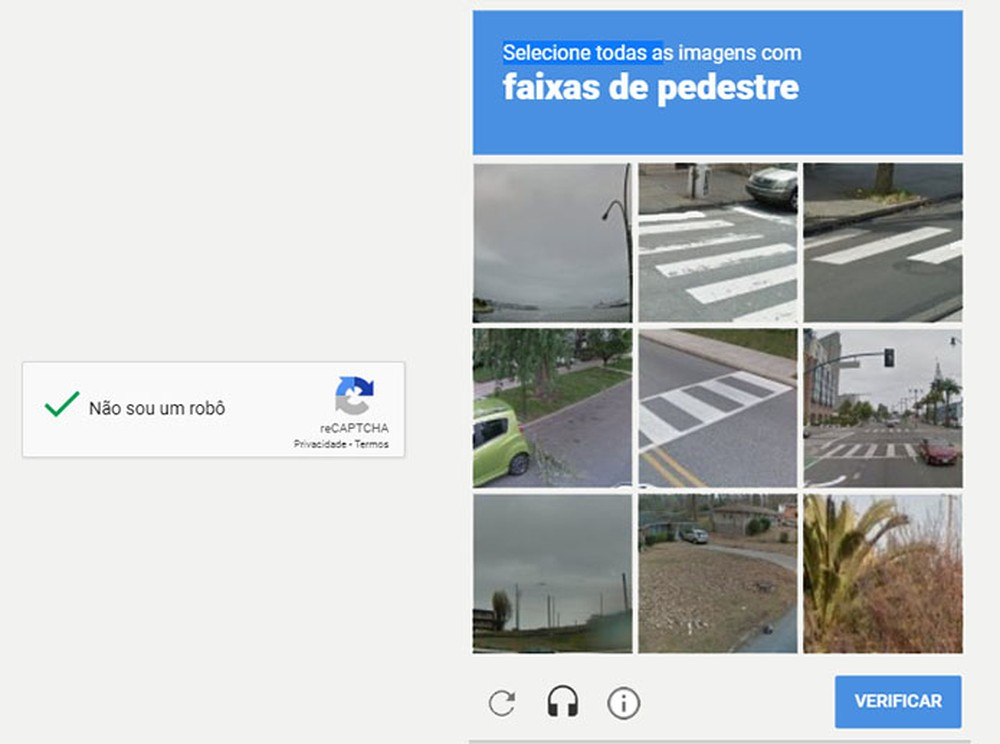
\includegraphics[scale=0.15]{tcc/figures/captcha/recaptcha-post-g1.jpg}
    \caption{Exemplo de um CAPTCHA moderno}
    \label{fig-exemplo-captcha-alfanumerico}
\end{figure}

\section{A Nota Fiscal de Consumidor Eletrônica}\label{secNfce}

A Nota Fiscal de Consumidor Eletrônica (NFC-e) visa ser uma alternativa eletrônica aos antigos cupons fiscais emitidos em papel. Tal documento segue um modelo nacional de emissão de documento fiscal com validade jurídica garantida pela assinatura digital do emissor.

Com a publicação do Decreto nº 44.785 em 12 de maio de 2014, a NFC-e foi instituída no Estado do Rio de Janeiro a partir do dia seguinte à publicação. Com isso, todos os estabelecimentos comerciais deveriam estar aptos ao uso da NFC-e até o dia 31 de dezembro de 2017.

% FIXME: Ajustar a imagem
% FIXME: Adicionar referencia a imagem
\begin{figure}[h]
    \centering
    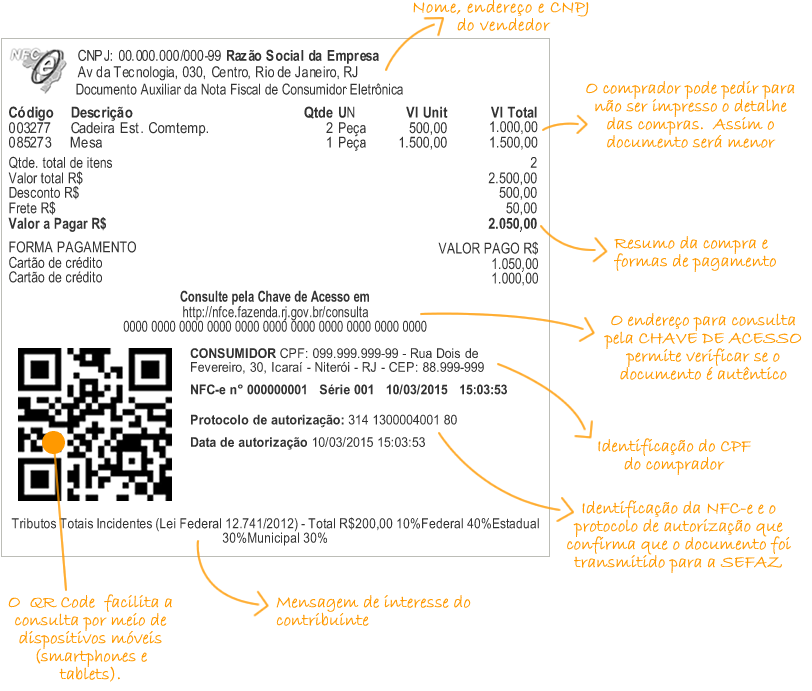
\includegraphics[scale=0.5]{modelo_nota_fiscal}
    \caption{Exemplo de uma NFC-e}
    \label{modeloNfce}
\end{figure}

Na figura \ref{modeloNfce} é possível observar um exemplo de uma NFC-e, com isso, pode se observar a descrição, a quantidade e o preço unitário de cada produto comprado. Além disso, ainda consta a informação do estabelecimento onde a compra foi efetuada como o endereço, o CNPJ e nome do estabelecimento.

Ainda, nesse documento consta uma chave de acesso que é composta por 44 dígitos e um QRCode, de posse desses dados é possível acessar a versão online da respectiva nota, no qual contém as mesmas informações a respeito da compra assim como existe em sua versão física.

% TODO: Adicionar print imagem nota online?

A verificação de autenticidade pode ser efetuada através de um site disponibilizado e mantido por cada Secretaria de Fazenda dos estados que constituem a União. Sendo assim, não é possível verificar a autenticidade de uma NFC-e emitida no estado de São Paulo na plataforma disponibilizada pelo Secretaria de Fazenda do Estado do Rio de Janeiro.